\documentclass[a4paper,11pt]{article}

\title{Intelligent Multimedia Systems\\Mean-Shift Object Tracking}
\author{J. v. Turnhout (0312649) \& R. Tobi (0448710)}

\usepackage{amsmath}
\usepackage{amsfonts}
\usepackage{graphicx}
\usepackage{float}
\usepackage{algorithm}
\usepackage{algorithmic}
\newcommand{\tbf}{\textbf}
\newcommand{\ds}{\displaystyle}
\newcommand{\ra}{\rightarrow}

%% To complete this course you must pass the exam and hand in a report
%% describing the work you did for this lab. Together with this report
%% you'll hand in your code and some illustrative result videos and still
%% images. Instead of mailing multi-gigabyte video documents, you should
%% put them somewhere in your web site (public_html) and  the link to me.
%%
%% Note that the most important part is to implement the tracker in a correct
%% way. After you made sure your implementation is correct, try the tracker on
%% a video in a different domain (search on the internet to find a good video
%% or create your own video). Keep in mind that when looking for a suitable
%% video, the goal is not to show how good the tracker works, but try to put
%% your finger on the strong and weak parts of the algorithm. After you analyzed
%% these strong and weak points of the algorithm, try to come up with suggestions
%% to improve your design. If there is still enough time, you can implement one
%% or more of your suggestions and analyze the results (for instance, how does
%% your improvement compare to the original algorithm with respect to the weak
%% as well as the strong parts of the original algorithm). If you run out of
%% time, you can describe how you would change the design and explain your
%% expectations of this change. 
%%
%%
%% The report should be about 10 pages long. This should be long enough
%% to give a thorough description of your work, including introduction,
%% conclusions and a discussion. In a paper-style report, the introduction
%% would consist of a problem description (object tracking) and some related
%% work (mention some approaches taken by other researchers, you can use
%% the reader for this or look some up yourself). Then, give an outline
%% of the approach that you have taken (mean-shift and color histograms).
%% Describe the used algorithm and features in you own words. In the next
%% sections, you can write about your implementation and the experimental
%% results. Make sure to mention all relevent issues that you have done
%% and why. For instance, make mention of your approach to color, which
%% color model and why. When writing this part, keep in mind that a reader
%% should be able to reproduce your results by using the information in this
%% report. After that, give a detailed report of the results of your tracker,
%% including graphs and screenshots. In the final section(s), you can give a
%% discussion of your results, in which you can comment on the tracking results
%% and introduce improvements that you have thought of. Furthermore, describe
%% what the effects of your improvement are, or, for lack of time, describe
%% what you expect the effects of the proposed improvements would be. Mention
%% things like processing speed (and possible improvements), the handling of
%% different domains (is one general solution possible, should the tracker be
%% adapted for each domain, how will the adaptation be done, etc.). Don't forget
%% to include your references at the end, and cite your sources in the text.

\begin{document}
	\maketitle

	\abstract{
		\noindent
		We implement a mean-shift tracker in \verb|MATLAB| for following objects in
		video and evaluate it on three different domains. The tracker's theoretical
		underpinnings are described and we explore weaknesses in its design.
	}

	\section{Introduction}
		Robust real-time tracking of objects in a sequence of video frames is one of
		the core problems of computer vision. A target object needs to be localized
		and represented in such a way as to be insensitive to changes in illumination,
		rapid movement, occlusion conditions, cluttering, background appearance, and
		scale. Furthermore, the per-frame computations should take no more than $100$
		milliseconds to be useful for real-time applications. These challenging
		conditions have led to many different approaches, most probabilistic in
		nature.
		\\ \\
		To track an object, we must iteratively establish its position in subsequent
		frames based on a known initial position. The essential step is then to create
		a target representation, such as a histogram, and attempt to find the position
		that best matches this representation in the next frame(s). If the tracker
		employs a brute-force algorithm, we may only exploit temporal locality in
		this matching step; that is, we assume the object's new position will be
		``close to'' its old one and search outwards in eg. a radial pattern. Such
		a brute-force tracker does no more than comparing the histogram $h_{x,y}^{w,h}$
		centered at each pixel $(x, y)$ with search-window dimensions $(w, h)$ to
		the target object histogram $h_{O}$ specified beforehand. Although this
		approach can be parallelized, the computational complexity renders it
		generally infeasible for larger windows.
		\\ \\
		A more efficient strategy is to incorporate kernel-weighted histograms.
		Each histogram pixel is now assigned a weight by a kernel mask based on
		its distance from the center-point. Because pixels further from the
		center of the tracked object will be the first to become occluded or
		warped under transformation, their values are less reliable. A kernel
		also imposes a ``smooth'' distance metric over histograms, which is
		required for the mean-shift step discussed below. The target's center
		pixel acts as the reference point; thus, the window width and height
		need to be odd. The efficiency gain comes from the fact that we can
		now steer the tracker towards the object's most likely new position
		by following the gradient rather than by examining all pixels within
		the local environment. This new position is derived from the histogram
		whose Bhattacharyya distance to the target's histogram representation
		is smallest.
		\\ \\
		%% The mean-shift tracker is a special case of the kernel-based tracker.
		%% Instead of doing a brute force search of all surrounding pixels, a gradient
		%% method is used to efficiently move towards the new position of the target.
		%% The new position of the target will of course be the positions of the candidate
		%% histogram with the smallest distance from the target. But we won't calculate
		%% the distance for all pixel positions, we will do it in an iterative fashion,
		%% starting from the last known position.
		%% KOEN:
		%% The mean-shift algorithm requires that we use a certain class of kernels for
		%% our kernel based histograms, only for this class the algorithm has been proved
		%% to converge (in most cases). So we need to calculate the Epanechnikov kernel.
		%% The formula is in the paper, but you will need these constants: $d = 2, c_d = \pi$.
		%% In my implementation I calculate the kernel beforehand and store the values in a
		%% matrix the size of the target region. This way I can look up the weight of a pixel
		%% with one look in the kernel matrix.
		%% The mean-shift step looks quite complicated, but is essentially easy to implement,
		%% once you know what is going on. It calculates the step that has to be taken from
		%% the current position towards the new position. The next step in the mean-shift
		%% algorithm is a little trick to compensate for too large mean-shift steps. Occasionally
		%% the calculated step is too large, the next step would of course move (back) towards
		%% the optimal position, but mean-shift calculations are expensive. Therefore it is
		%% efficient to correct for the overshoot and this step does just that. It picks a
		%% point between the previously and newly calculated position and sees if that point
		%% is a better match (compare histograms) than the calculated position. If it is the
		%% position half-way is chosen and the process is repeated. This will correct overshoot
		%% without needing another mean-shift step.
		%% \\ \\
		%% The basis of the mean-shift tracker is a kernel-based histogram creation function.
		%% You will need to implement this. This function takes a position or offset as parameter
		%% and will then calculate the histogram for an area of width x height pixels. This means
		%% finding the proper bin for each pixel and looking up the weight from the kernel function
		%% (see Lab 8), this weight is then added to the calculated bin. This function needs to be
		%% completed before you can start on the mean-shift tracker. Note: these kernel weights
		%% mentioned here are values of the kernel function k(). Assuming that this weight is w
		%% would be a mistake.
		%% \\ \\
		%%
		In the tracking phase we calculate the kernel-based histogram for the target during
		each frame $f$. Then for each new frame we calculate the \textit{candidate} histogram
		centered at the target's last known position. A combination of equations $10$ and $13$
		from \cite{KBOT} over a window of size $(w, h)$ then produces the new location estimate
		$(x_{f+1}, y_{f+1})$. This gives us the \textit{mean-shift} from which the tracker's name
		is derived. However, a limitation of the algorithm is that this shift can sometimes exceed
		the target, taking many extra iterations to be re-aligned. A practical hack to avoid this
		problem as mentioned in \cite{KBOT} is to check whether the histogram at the position halfway
		between the object's old position and the new estimate is a better match in terms of the
		Bhattacharyya distance.
		\\ \\
		The remainder of this paper is organized as follows. Section $2$ outlines the mathematical
		foundations of the mean-shift tracker in detail. Section $3$ relates this theory to our
		\verb|MATLAB| implementation and issues we encountered. We evaluate our tracker and present
		results in section $4$, and conclude in section $5$. Finally, section $6$ offers some directions
		for future work.
		%%
		%% After performing this formula, you have the mean-shift, the amount you need to adapt your
		%% position to move closer to the target. The following step in the paper is sort of a hack
		%% to compensate for too large shifts. The algorithm sometimes calculates a step that will
		%% move beyond the target. Subsequent mean-shift steps will lead to the optimal position,
		%% but it is computationally cheaper to solve this in another way: See if the position halfway
		%% between the calculated new position and the original position is a better match (Bhattacharyya),
		%% if it is: take this position as new position and repeat.
		%% \\ \\
		%% One final issue regarding the processing of the frames is this. In lab 6, I gave a little
		%% piece of code to read the frames subsequently. The whole idea of tracking is, that you try
		%% to track a player in MULTIPLE frames. So, do not stop after one or two frames, but see how
		%% your algorithm handles several frames in a row. Ideally, you would process all subsequent
		%% frames, but if this takes too long, you could consider to skip some (one or two) frames
		%% after processing a frame, eg. after processing frame x, continue with frame (x+1); however,
		%% if it takes too long, then skip frame (x+1) and continue with frame (x+2). However, please
		%% keep in mind that tracking does not stop after one frame! See what happens if you track a
		%% player over several seconds of video.
		%% \\ \\
		%% After processing the frames, it would be nice to see the results of your tracking algorithm.
		%% You can do this by painting a rectangle in a frame on the new position and write this image
		%% to disk. However, Matlab also provides the possibility to create an avifile from your frames.
		%% The matlab-function to do this is called \verb|avifile|. 

	\section{Theoretical Background}
		Two components can be distinguished in a tracker; the \textit{Object Model}
		and the \textit{Tracking Model}. The first is concerned with localizing and
		representing the type of object to be tracked up from the individual pixels,
		while the second deals with the high-level task of filtering to describe object
		motion.
		FIXME: TOO VAGUE?
		In abstract terms, this process of filtering can be modelled as a discrete-time
		dynamical system through the well known state-space approach. Each state $x_k$
		(for $k=0, 1, ...$) characterizes the relevant information about the tracked
		object, and dynamically evolves over time according to $x_k = f_k(x_{k - 1}, v_k)$
		where $v_k$ is the $k$-th (i.i.d) noise item. The states are not directly observable;
		rather a sequence of measurements $\{z_k\}$ evolving via $z_k = h_k(x_k, n_k)$
		(with $\{n_k\}$ another i.i.d noise sequence) provides ``hints'' about the true
		state at each time-step $k$, which is a latent variable. The tracker's task
		is now to estimate $x_k$ given all preceding measurements $z_{1:k}$, ie. it
		must recover the unknown probability density function $P(x_k \mid z_{1:k})$.
		This formulation leads to the general technique of recursive Bayesian estimation,
		which assumes the states $\{x_k\}$ and observations $\{z_k\}$ to be the hidden
		and visible parts of a hidden Markov model (HMM). The RBE method constructs the
		p.d.f in a prediction and an update step conceptually similar to those of the
		Expectation-Maximization algorithm family. When $v_k$ and $n_k$ are Gaussian
		and the prediction and update functions $f_k$ and $h_k$ are (non-)linear, the
		estimator becomes an instance of the (Extended) Kalman filter. However, other
		filter classes can also be used.
		\\ \\
		The mean-shift tracker assumes only small changes in location and appearance
		of the target object between two consecutive frames. This enables an efficient
		gradient-based localization scheme. Specifically, the target object is spatially
		masked with an isotropic kernel, which allows us to define a smooth similarity
		function and reducing the localization problem to a search in this function's
		basin of attraction (ie., all points in the state-space that enter the same
		region $R$ over time). The MST's object model is given by a histogram in some
		color-space. This is a non-parametric color density estimate, extracted both
		for the target-object model (p.d.f) $q$ and for the per-frame target-object
		candidates $p(\tbf{v})$; where $\tbf{v} = (x, y)$. The similarity function
		between histograms $p$ and $q$ is abstractly denoted by $\rho[p(\tbf{v}), q]$.
		This function is regularized by applying an isotropic spatial Epanechnikov kernel
		to the objects so that large variations in spectral information for adjacent image
		pixels are suppressed and continuous spatial data is retained, allowing the use of
		gradient-based methods to search for its maxima.
		\\ \\
		The Bhattacharyya distance measures the similarity of two discrete or continuous
		probability distributions. It is related to the Bhattacharyya coefficient, which
		measures the amount of overlap between two statistical sample-sets. The coefficient
		can be used to determine the relative closeness of two given samples; in our case,
		histograms. For continuous distributions, the coefficient is defined as
		$\rho[p, q] = \int \sqrt{p(x) \cdot q(x) } \delta x$, $0 \leq \rho \leq 1$.
		Calculating the Bhattacharyya coefficient involves integration of the overlap
		of the two samples. The interval of the values of the two samples $a$ and $b$
		is split into a chosen number of discrete bins $n$, and the number of members
		$a_i$ and $b_i$ of each sample in each bin $i$ summed according to
		$\sum_{i=1}^{n} \sqrt{\Sigma a_i \cdot \Sigma b_i}$. Each partition that contains
		members from both samples contributes to the coefficient, as do partitions that
		share a large degree of overlap of the members of the two samples  within it. The
		choice of $n$ depends on the number of members in $a$ and $b$; too few partitions
		will incur loss of accuracy by over-estimating the region of overlap, while too many
		will also reduce the accuracy due to under-estimation. From $\rho$, the Bhattacharyya
		\textit{distance} is determined by $d = \sqrt{1 - \rho[p, q]}$.
		%% This is better than straight Euclidean distance because of FIXME.


	\section{Implementation}
		The core of the implementation of the tracker follows the algorithm described
		in \cite{KBOT} closely, but with some small changes.
		\\ \\
		%% We implement the Epanechnikov weight-function by pre-calculating a 2D
		% table of kernel values equal in size to the target region, which stores
		%% the weight for each relative pixel position. We add the weight per pixel
		%% to the corresponding histogram bin via a single lookup into this table.
		%% NOTE: DOES THE CODE ACTUALLY DO THIS?
		The target model is represented by a kernel-weighted histogram. We implement
		the Epanechnikov weight-function by pre-calculating a 2D table of kernel values
		equal in size to the target region which stores the weight for each relative pixel
		position. We add the weight per pixel to the corresponding histogram bin via a single
		lookup into this table. The target region is scaled to unit height and width as well
		as any future candidate region, therefore the kernel needs to be calculated only once
		beforehand.
		\\ \\
		The weights needed to calculate the eventual shift are given by equation ($10$)
		from \cite{KBOT} and can be calculated at once using a back projection approach.
		By calculating $H=\sqrt{\frac{M}{H_0}}$, where $M$ is the target model and $H_0$
		is the candidate histogram, the weights are stored in a histogram. Now it is
		possible to use back-projection on this new histogram $H$ and the image patch
		$P_0$ to set the corresponding weight for every pixel in the image patch by
		using the histogram $H$ as a lookup table.
		\\ \\
		With the weights calculated, the shift from the current position to a new position
		is derived by summing over the products of the positions relative from the center
		of the image patch and their corresponding weights (line 18 in algorithm \ref{alg:MST}).
		This shift however can be too large, and the new position can pass the real position
		of the object. A method to deal with large shifts is to iteratively reduce the distance
		between the old position and the new position by a factor of $\frac{1}{2}$ until the
		condition $\rho_{H_1} < \rho_{H_0}$ is met, where $\rho_{H_x}$ is the Bhattacharyya
		distance between the target candidate histogram $H_x$ and the target model $M$.
		\\ \\
		The final step in the implementation is the acceptation or rejection of the new
		position with respect to the old position. In our implementation we set the condition
		to the norm of the new minus the old position to be zero in order to accept the new
		position. If this is not the case, the new position is used in a recursive call to
		the \verb|MeanShiftRecursive| function. The depth of recursion is constrained to a
		maximum of $4$ steps to keep reasonable speed and in practice this depth gives good
		results.
		\\ \\
		Since caching all the frames of our animation test-sequences prior to
		tracking would cost a prohibitive amount of memory, we read each frame
		incrementally from disk on an as-needed basis. However, this reduces
		performance. Ideally, for any given frame number, we would pre-load the
		next $n$ frames in a separate thread, but \verb|MATLAB| provides no such
		facilities.
		\\ \\
		A pseudo-code global overview of the tracker is included below.
		\subsection{Algorithm}
			\begin{algorithm}[H]
				\caption{Mean-shift Tracker}
				\begin{algorithmic}[1]

				\STATE {\tbf{function} MeanShift\_Tracker($D$,$M$)}
				\STATE {$D$ = Image Sequence}
				\STATE {$M$ = Target Model}
				\medskip
				\STATE {$K \leftarrow$ Epanechnikov Kernel}
				\STATE {$center \leftarrow$ Starting Position}
				\FOR {$d \epsilon D$}
					\STATE {DrawRectangle($d$,$center$)}
					\STATE {$center \leftarrow$ MeanShiftRecursive($M$,$d$,$center$,$K$, $0$)}
				\ENDFOR
				\medskip
				\STATE {\tbf{function} MeanShift\_Recursive($M$,$d$,$center$,$K$, $Iter$)}
				\STATE $P_x$ = Candidate Image Patch $x$
				\STATE $H_x$ = Candidate Histogram $x$
				\STATE $x_i$ = pixel-location in image patch relative to the center
				\STATE $\rho_{H_x} = \sqrt{H_x \cdot M}$
				\medskip
				\STATE $H_0 \leftarrow$ Histogram($d$,$center$,$K$)
				\STATE $P_0 \leftarrow$ ImagePart($d$, $center$)
				\STATE $\tbf{w} \leftarrow$ BackProjection($P_0$, $\sqrt{\frac{M}{H_0}}$)
				\STATE $newCenter \leftarrow \frac{\sum_i^n x_iw_i}{\sum_i^n w_i} + center$
				\STATE $H_1 \leftarrow$ Histogram($d$,$newCenter$,$K$)
				\WHILE{$\rho_{H_1} < \rho_{H_0}$}
					\STATE $newCenter = \frac{1}{2} \cdot (center + newCenter)$
					\STATE evaluate $\rho_{H_1}$
				\ENDWHILE

				\IF {$\parallel newCenter - center \parallel > 0$ or $Iter<4$}
					\STATE $newCenter \leftarrow$ MeanShiftRecursive($M$,$d$,$newCenter$,$K$, $Iter+1$)
				\ELSE
					\STATE \tbf{return} $newCenter$
				\ENDIF
				\end{algorithmic}
				\label{alg:MST}
			\end{algorithm}
			\noindent
			Of crucial importance to the implementation is the selection of the right
			color-space for the target-object model. The color-space is a major factor
			in determinining the tracker's discriminative ability based on whether it
			is sensitive to illumination changes (eg. color and direction), specular
			highlights, radiant intensity, object geometry and surface orientation,
			and other properties. Very often the ``best''\footnote{In so far as this
			can be objectively established.} color-space is also dependent on the
			domain of interest. For example, when tracking brightly-colored soccer
			players moving across the field (a large diffuse grass surface), the
			normalized-RGB system will be better capable of discriminating fore-
			and background pixels than the RGB system from which it originates.
			Figure \ref{fig:CORAL} illustrates this as well.
			\\ \\
			We evaluate our tracker in the \verb|RGB|, \verb|rgb|, \verb|HSV|, and
			\verb|OSC| spaces. The object model is then a $2D$ (\verb|rgb|) or $3D$
			(\verb|RGB|, \verb|HSV|, \verb|OSC|) histogram respectively. The number
			of bins per histogram is not a function of the number of dimensions, ie.
			each dimension contains $N^{\frac{1}{d}}$ bins ($d \in \{2, 3\}$) of width
			$16$ where $N$ is the total bin-count. For a detailed overview of the various
			color-spaces, we refer to \cite{COLOR}.

		%% Histogram distances
		%% To check the result you get from the object detection and to maybe choose
		%% between several detected objects, you can compare the histograms of the
		%% target and the candidate objects. So you create a histogram for the candidate
		%% objects in exactly the same fashion as you did for the target. Now you need
		%% to compare the candidate and target histogram, in some meaningful way. The
		%% reader (available on Blackboard and for sale in paper form as well) discusses
		%% several methods. I will repeat two here:
		%% \\ \\
		%% Euclidean distance: The Euclidean distance between histograms calculates the
		%% following distance between all histogram bins: $(b1 - b2)^2$, then sums this
		%% over all bins and takes the square root.
		%% \\ \\
		%% Bhattacharyya distance: The Bhattacharyya distance is a measure to compare
		%% statistical distributions, something that our histograms represent. The
		%% Bhattacharyya distance is calculated as follows. First the Bhattacharyya
		%% coefficient is determined by $\rho[p, q] = \int \sqrt{p(u) \cdot q(u) } \delta u$,
		%% then the Bhattacharyya distance is determined from this by $d = \sqrt{1 - \rho[p, q]}$.
		%%
		%% LaTeX is the typesetting system, which has (amongst others) the two compilers
		%% latex and pdflatex. The first one produces DVI output, the second has PDF as
		%% output format. latex only accepts PS/EPS files for graphics inclusion. pdflatex
		%% accepts JPG, PNG and finally PDF format.
		\begin{figure}[H]
			\begin{center}
				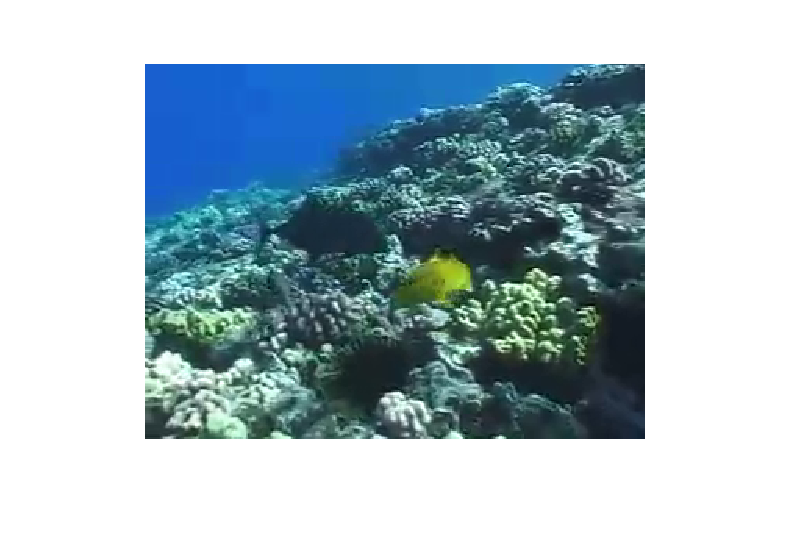
\includegraphics[width=8cm]{img/cs_RGB.eps}\\
				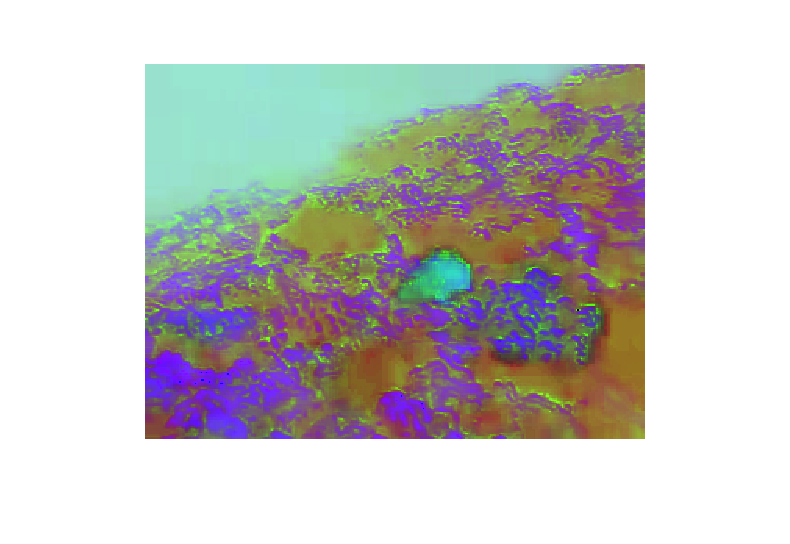
\includegraphics[width=4cm]{img/cs_HSV.eps}
				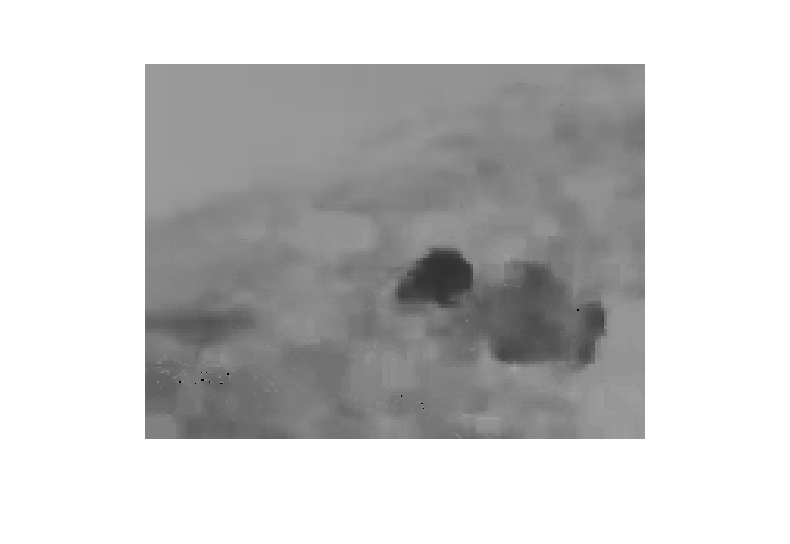
\includegraphics[width=4cm]{img/cs_Hue.eps}\\
				
\includegraphics[width=4cm]{img/cs_nRGB.eps}
				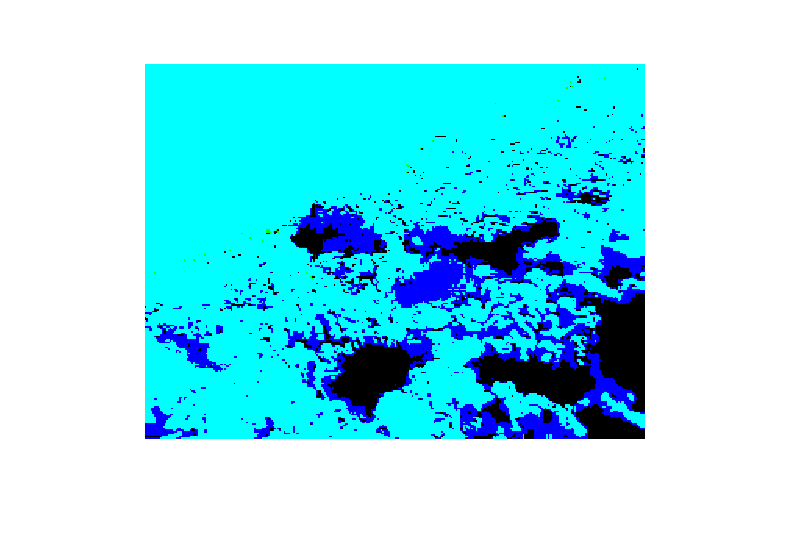
\includegraphics[width=4cm]{img/cs_OCS.eps}
			\end{center}
			\caption{
				Coral, represented in five different color-spaces. Top image:
				RGB. Bottom image quadrant in clockwise order: HSV, Hue, OCS,
				and rgb. The tropical fish in front of the reef is almost
				invisible in OCS, yet clearly visible in HSV.
			}
			\label{fig:CORAL}
		\end{figure}

	\section{Evaluation and Results}
		%% KOEN: If you think your tracker is finished, you can think about how to evaluate
		%% the performance of your tracker. Further, you can think about the strong and
		%% weak parts of your tracker, and propose possible improvements. If there is
		%% enough time, you can implement one or more of your proposed improvements and
		%% analyse the effect compared to the original tracker.
		%% \\ \\
		%% Once you think you completed the mean-shift tracker, it is time to test your
		%% implementations on videos from different domains and analyze the performance
		%% of different color spaces. What are the advantages and disadvantages of certain
		%% color spaces, when do you think you should use one color space instead of the
		%% other, etc. After that, you can think about improvements of the tracker. This
		%% involves a thorough analysis of your current version, including an analysis of
		%% the strong and weak points. If you know when your tracker goes wrong, you can
		%% think of possible solutions to overcome these difficulties.
		%% \\ \\
		%% However, first think about how to evaluate the performance of your tracker. It
		%% would be nice to show some quantitative results in your report, instead of pointing
		%% at the videos and stating ``Look, it works!''. Several options exist, some more
		%% time-consuming than others. Come talk to me if you have no clue on how to proceed
		%% with this.
		%% \\ \\
		%% If you finished your tracker, and thought about how to evaluate it, then it is
		%% time to test your tracker on videos from different domains. For this, you can
		%% use the Internet to download videos or capture your own. For the conversion of
		%% your videos into frames, I suggest you use the linux-program mplayer. Matlab can
		%% also handle video-files, but you will get memory problems if you use videos that
		%% are longer than a couple of seconds.
		%% \\ \\
		%% Note that the most important part is to implement the tracker in a correct way.
		%% After you made sure your implementation is correct, try the tracker on a video
		%% in a different domain (search on the internet to find a good video or create your
		%% own video). Keep in mind that when looking for a suitable video, the goal is not
		%% to show how good the tracker works, but try to put your finger on the strong and
		%% weak parts of the algorithm. After you analyzed these strong and weak points of
		%% the algorithm, try to come up with suggestions to improve your design. If there
		%% is still enough time, you can implement one or more of your suggestions and analyze
		%% the results (for instance, how does your improvement compare to the original algorithm
		%% with respect to the weak as well as the strong parts of the original algorithm). If
		%% you run out of time, you can describe how you would change the design and explain your
		%% expectations of this change.
		Evaluation of the tracker is not a trivial task where we are provided with a ground-truth
		to use for measuring the performance of the tracker. Since we are interested in the various
		pros and cons of the tracker we conducted experiments on several domains. For our experiments
		we chose three different domains: sport, urban and nature. For each of these domains we use
		two different environments within the domain and conduct a tracking experiment for each color
		space described earlier. To test the robustness on these domains we do need some constraints
		within the videos themselves. The most important constraint is that the target is not fully
		occluded during tracking, since the tracker cannot handle this in our implementation. Another
		important constraint to the videos is that there should not be any cuts to different cameras
		in the movie when tracking the object. Since mean-shift tracks the object from frame to frame,
		it cannot handle tracking objects that appear in totally different locations when having a cut
		from camera to camera. A final constraint is that the object should not scale too much. The
		tracker can deal with some scaling but the tracker patch does not grow or shrink when the object
		gets scaled. The evaluation criterion is simple: for each video and for each color space, we test
		whether it is possible to track a certain object for the entire sequence of frames.
		\begin{table}[H]
			\centering
			\begin{tabular}{ | l | l | l | l | l | l |}
			\hline
			                   & RGB & rgb & OCS & HSV & Hue \\
			\hline
			Formula 1 (1):  97 & 1   & 1   & 0   & 0   & 1 \\
			Formula 1 (2): 215 & 1   & 0   & 0   & 0   & 0 \\
			Formula 1 (3): 123 & 0   & 0   & 0   & 0   & 1 \\
			Formula 1 (4): 222 & 0   & 0   & 0   & 0   & 1 \\
			Formula 1 (5): 164 & 1   & 0   & 0   & 1   & 1 \\
			\hline
			\end{tabular}
			\caption{}
		\end{table}
		\begin{table}[H]
			\centering
			\begin{tabular}{ | l | l | l | l | l | l |}
			\hline
			                   & RGB & rgb & OCS & HSV & Hue \\
			\hline
			Soccer (1): 201    & 1   & 1   & 0   & 1   & 1 \\
			Soccer (2): 164    & 1   & 1   & 0   & 1   & 1 \\
			Soccer (3): 223    & 0   & 0   & 0   & 1   & 1 \\
			Soccer (4): 186    & 0   & 0   & 0   & 0   & 0 \\
			Soccer (5): 239    & 0   & 0   & 0   & 0   & 0 \\
			\hline
			\end{tabular}
			\caption{}
		\end{table}
		\noindent
		The sporting domain gives us a more controlled environment for tracking. Formula $1$ is set on
		grey roads with green grass surrounding it, making it possible to track racecars with certain
		color schemes fairly easy. Tracking in the soccer domain also benefits from the environment of
		the players and their clothing. However, the controlled environment can also be of negative
		influence. For example, when tracking a Formula 1 car we observe that using only the hue gives
		the best tracking results in general. But when the target model consists of average hue values
		relative to the environment the tracker will not always be able to FIXME END OF SENTENCE?
		\\ \\
		The urban domain gives a more challenging environment since we can expect about anything in the
		scenery. For this domain we chose walking people and free-running people (an urban sport). Because
		urban environments have a huge variety in features such as source illuminations, occlusion, clutter
		and reflecting surfaces, the tracking results are much more dependent on the color spaces.
		\begin{table}[H]
			\centering
			\begin{tabular}{ | l | l | l | l | l | l |}
			\hline
			                            & RGB & rgb & OCS & HSV & Hue \\
			\hline
			Pedestrian-Walk    (1):  82 & 0   & 0   & 0   & 1   & 0 \\
			Pedestrian-Walk    (2):  42 & 0   & 0   & 0   & 1   & 0 \\
			Pedestrian-Walk    (3):  84 & 0   & 0   & 0   & 1   & 0 \\
			Pedestrian-FreeRun (1): 174 & 0   & 0   & 1   & 0   & 1 \\
			Pedestrian-FreeRun (2): 163 & 1   & 0   & 0   & 0   & 0 \\
			Pedestrian-FreeRun (3): 387 & 0   & 0   & 0   & 0   & 0 \\
			\hline
			\end{tabular}
			\caption{}
		\end{table}
		\begin{table}[H]
			\centering
			\begin{tabular}{ | l | l | l | l | l | l |}
			\hline
			                   & RGB & rgb & OCS & HSV & Hue \\
			\hline
			Fish    (1): 314   & 0   & 0   & 0   & 0   & 0 \\
			Fish    (2): 319   & 0   & 1   & 0   & 1   & 1 \\
			Fish    (3): 322   & 1   & 1   & 1   & 1   & 1 \\
			Leopard (1): 387   & 0   & 0   & 0   & 1   & 1 \\
			Leopard (2):  91   & 0   & 0   & 0   & 1   & 0 \\
			Leopard (3): 105   & 0   & 0   & 0   & 1   & 1 \\
			\hline
			\end{tabular}
			\caption{}
		\end{table}
		\noindent


	\section{Conclusion}

	\section{Future Work}
		We have several suggestions for extending the tracker skeleton.

		\begin{itemize}
		\item{
			\emph{Scale-invariance}: this could be accomplished by computing the
			Epanechnikov kernel for various scales and selecting the appropriate
			scale each frame by means of the Bhattacharyya distance.
		}
		\item{
			\emph{Color-space selection}: it should be possible to perform some
			variance analysis on the target histogram and determine which color
			space is best suited for the object model.
		}
		\item{
			\emph{Spatial discrimination}: dividing the kernel into several parts
			to store spatial information could make the tracker more discriminative.
		}
		\end{itemize}

	\begin{thebibliography}{2}
		\bibitem{KBOT}
			D. Comaniciu, V. Ramesh, P. Meer: \textit{Kernel-Based Object Tracking}
		\bibitem{COLOR}
			T. Gevers: \textit{Color in Image Search Engines}
	\end{thebibliography}

\end{document}









% je hebt een color space en zo'n domein als sport
% waarom werkt normalized RGB zo fijn op voetbal
%  Jasper:  en kan 't problemen opleveren bij een grijze achtergrond
% met grijze achtergrond bedoel ik dan f1 wegdek
%  Jasper:  en urban environments zijn erg lastig
% daarom wil je over 't algemeen zoveel mogelijk informatie van de target model opslaan
% daarom werken in die filmpjes hsv en RGB volgens mij 't beste
%  me:  wat ik wel kan zeggen zijn dingen als "in domains where large diffuse surfaces dominate, normalized RGB works well because of blablabla"
%  Jasper:  dat is zoiezo een inkoppertje
% maar we moeten de zwaktes ook aanstippen dus
%  me:  daar heb ik dus niet goed zicht op ;)
%  Jasper:  en dan met name dus over zaken waar geen enkele color space iets mee kan
% www.youtube.com/watch?v=_RviOAIqRyk
% www.youtube.com/watch?v=qgdimzQaTG8
